% Name: Hook lengths of a Young diagram
% Description: The Young diagram of the partition (4, 2, 1) with each box's hook length written in it, and the hook length formula counting its 35 standard Young tableaux.
% Tags: Young diagram, hook length formula, partitions, standard Young tableaux

\begin{tikzpicture}[every node/.style={font=\small}]
  % Hook of a box: the boxes to its right, below it, and itself; row 1 gives 6, 4, 2, 1, row 2 gives 3, 1, row 3 gives 1
  \foreach \r/\row in {0/{6,4,2,1}, 1/{3,1}, 2/{1}}
    \foreach \h [count=\c from 0] in \row {
      \draw[thick, fill=blue!8] (0.8*\c,-0.8*\r) rectangle ++(0.8,-0.8);
      \node at (0.8*\c+0.4,-0.8*\r-0.4) {\h};
    }
  % The hook of the corner box, drawn over it
  \draw[orange!85!black, line width=1.4pt, rounded corners=2pt] (0.08,-0.08) -- (3.12,-0.08) -- (3.12,-0.72) -- (0.72,-0.72) -- (0.72,-2.32) -- (0.08,-2.32) -- cycle;
  \node[anchor=west] at (3.8,-1.2) {$f^{(4,2,1)} = \dfrac{7!}{6 \cdot 4 \cdot 2 \cdot 1 \cdot 3 \cdot 1 \cdot 1} = \dfrac{5040}{144} = 35$};
\end{tikzpicture}
